
\mychapter{Implementation}
\vspace{0.5cm}

\subsection{Introduction}

This chapter presents the implementation of the proposed \textbf{Digital Admission Script Evaluation and Moderation System (DASEMS)}. The system was developed as a web-based platform to automate the workflow of descriptive admission script evaluation.

The implementation follows a modular architecture comprising a React frontend, Node.js and Express.js backend, MongoDB database, and a Python-based document processing service for PDF analysis and answer extraction. These components communicate through RESTful APIs to ensure efficient integration and scalability.

The system supports admission management, PDF processing, teacher assignment, evaluation, moderation, and result generation, while preserving human judgment during answer assessment. The following sections describe the development environment and implementation techniques used in the proposed system.


\subsection{Development Environment}

The proposed \textbf{Digital Admission Script Evaluation and Moderation System (DASEMS)} was developed using a modern full-stack technology stack suitable for web-based applications and document processing.

The frontend was implemented using \textbf{React 18} and \textbf{TypeScript}, while the backend was developed using \textbf{Node.js} and \textbf{Express.js}. \textbf{MongoDB} was selected as the primary database because of its flexible document-oriented architecture. A separate Python service built with \textbf{FastAPI} performs PDF processing, OCR, and image analysis using libraries such as \textbf{PyMuPDF}, \textbf{pdfplumber}, \textbf{Pillow}, and \textbf{Tesseract OCR}.

Docker Compose was used to containerize the backend, database, Redis cache, and Python processing service, ensuring consistent deployment across different environments. Git was used for version control, while Visual Studio Code served as the primary development environment.


\begin{table}[ht]
\centering
\caption{Summarizes the technologies used during system development.}
\label{tab:development_environment}

\begin{tabular}{|p{5cm}|p{7cm}|}
\hline
\textbf{Component} & \textbf{Technology Used} \\
\hline
Programming Language & TypeScript, JavaScript, Python \\
\hline
Frontend Framework & React 18 \\
\hline
Backend Framework & Node.js, Express.js \\
\hline
Database & MongoDB \\
\hline
Document Processor & Python FastAPI \\
\hline
OCR Engine & Tesseract OCR \\
\hline
PDF Processing & PyMuPDF, pdfplumber \\
\hline
Image Processing & Pillow \\
\hline
Authentication & JWT, bcrypt \\
\hline
State Management & Redux Toolkit \\
\hline
API Communication & React Query \\
\hline
Styling & Tailwind CSS \\
\hline
Annotation Library & React Konva \\
\hline
Containerization & Docker Compose \\
\hline
Version Control & Git \\
\hline
Development Environment & Visual Studio Code \\
\hline
\end{tabular}
\end{table}

The complete system was developed and tested on a macOS environment, with Docker Compose managing communication among all services to provide a consistent and reliable development platform.

\subsection{Backend Implementation}

The backend is the core component of the proposed \textbf{Digital Admission Script Evaluation and Moderation System (DASEMS)}. It manages communication among the frontend, MongoDB database, and Python document processing service while implementing the system's business logic.

Developed using \textbf{Node.js} and \textbf{Express.js}, the backend follows a modular architecture with controllers, services, repositories, models, and middleware. It supports authentication, student and admission management, answer script processing, teacher assignment, evaluation, moderation, and reporting.

The following subsections describe the backend structure, authentication mechanism, and REST API implementation.


% flow chart
%===========================
% Preamble
%===========================

\usetikzlibrary{positioning,arrows.meta,calc}

%===========================
% Figure
%===========================
\begin{figure}[ht]
\centering
\resizebox{\textwidth}{!}{%
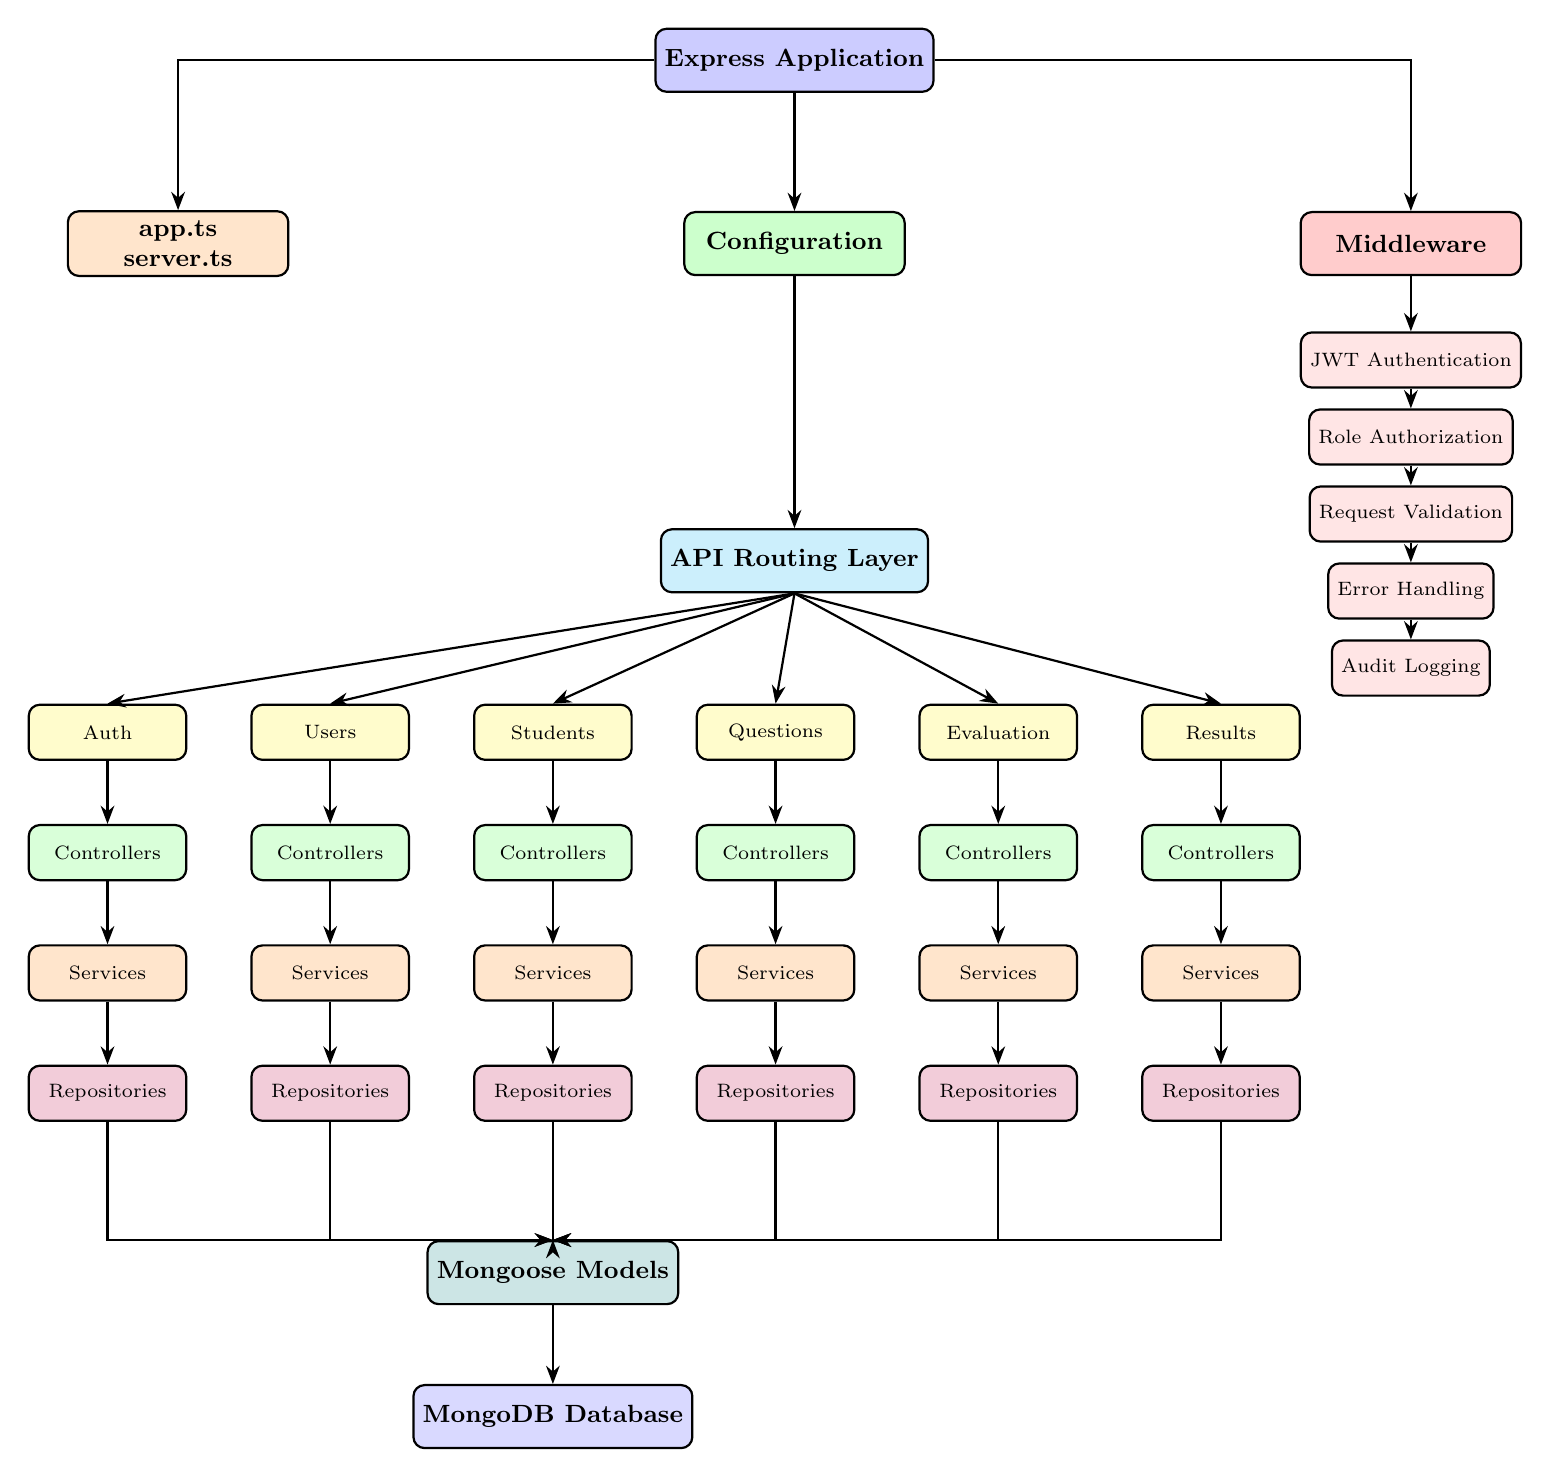
\begin{tikzpicture}[
    >=Stealth,
    node distance=1cm,
    box/.style={
        draw,
        rounded corners,
        thick,
        minimum width=2.8cm,
        minimum height=0.8cm,
        align=center,
        font=\small\bfseries
    },
    smallbox/.style={
        draw,
        rounded corners,
        thick,
        minimum width=2cm,
        minimum height=0.7cm,
        align=center,
        font=\scriptsize
    },
    arrow/.style={->,thick}
]

%------------------------------------------------
% Top Layer
%------------------------------------------------

\node[box,fill=blue!20] (app) {Express Application};

\node[box,fill=green!20,below=1.5cm of app] (config) {Configuration};

\node[box,fill=orange!20,left=5cm of config] (server)
{app.ts\\server.ts};

\node[box,fill=red!20,right=5cm of config] (middleware)
{Middleware};

\draw[arrow] (app) -- (config);
\draw[arrow] (app) -| (server);
\draw[arrow] (app) -| (middleware);

%------------------------------------------------
% Middleware
%------------------------------------------------

\node[smallbox,fill=red!10,below=0.7cm of middleware] (jwt)
{JWT Authentication};

\node[smallbox,fill=red!10,below=0.25cm of jwt] (role)
{Role Authorization};

\node[smallbox,fill=red!10,below=0.25cm of role] (req)
{Request Validation};

\node[smallbox,fill=red!10,below=0.25cm of req] (err)
{Error Handling};

\node[smallbox,fill=red!10,below=0.25cm of err] (audit)
{Audit Logging};

\draw[arrow] (middleware)--(jwt);
\draw[arrow] (jwt)--(role);
\draw[arrow] (role)--(req);
\draw[arrow] (req)--(err);
\draw[arrow] (err)--(audit);

%------------------------------------------------
% Router
%------------------------------------------------

\node[box,fill=cyan!20,below=3.2cm of config] (router)
{API Routing Layer};

\draw[arrow] (config)--(router);

%------------------------------------------------
% Modules
%------------------------------------------------

\node[smallbox,fill=yellow!20,below left=1.4cm and 6cm of router] (auth){Auth};
\node[smallbox,fill=yellow!20,right=0.8cm of auth] (users){Users};
\node[smallbox,fill=yellow!20,right=0.8cm of users] (students){Students};
\node[smallbox,fill=yellow!20,right=0.8cm of students] (questions){Questions};
\node[smallbox,fill=yellow!20,right=0.8cm of questions] (evaluation){Evaluation};
\node[smallbox,fill=yellow!20,right=0.8cm of evaluation] (results){Results};

\foreach \x in {auth,users,students,questions,evaluation,results}
\draw[arrow] (router.south)--(\x.north);

%------------------------------------------------
% Controllers
%------------------------------------------------

\foreach \x/\name in {
auth/authc,
users/usersc,
students/studentsc,
questions/questionsc,
evaluation/evaluationc,
results/resultsc}
{
\node[smallbox,fill=green!15,below=0.8cm of \x] (\name)
{Controllers};

\draw[arrow] (\x)--(\name);
}

%------------------------------------------------
% Services
%------------------------------------------------

\foreach \x/\name in {
authc/auths,
usersc/userss,
studentsc/studentss,
questionsc/questionss,
evaluationc/evaluations,
resultsc/resultss}
{
\node[smallbox,fill=orange!20,below=0.8cm of \x] (\name)
{Services};

\draw[arrow] (\x)--(\name);
}

%------------------------------------------------
% Repositories
%------------------------------------------------

\foreach \x/\name in {
auths/authr,
userss/usersr,
studentss/studentsr,
questionss/questionsr,
evaluations/evaluationr,
resultss/resultsr}
{
\node[smallbox,fill=purple!20,below=0.8cm of \x] (\name)
{Repositories};

\draw[arrow] (\x)--(\name);
}

%------------------------------------------------
% Database
%------------------------------------------------

\node[box,fill=teal!20,below=1.5cm of studentsr]
(mongoose){Mongoose Models};

\node[box,fill=blue!15,below=1cm of mongoose]
(mongo){MongoDB Database};

\foreach \x in {authr,usersr,studentsr,questionsr,evaluationr,resultsr}
{
\draw[arrow] (\x.south)|-(mongoose.north);
}

\draw[arrow] (mongoose)--(mongo);

\end{tikzpicture}
}
\caption{Express Backend Architecture}
\label{fig:express_backend}
\end{figure}

\subsubsection{Project Structure}

The backend follows a feature-oriented directory structure, where related files are grouped into independent modules for easier maintenance and future expansion.

The main directories are:

\begin{itemize}
\item \textbf{Config}: Configuration and database settings.
\item \textbf{Routes}: REST API endpoints.
\item \textbf{Controllers}: Request handling.
\item \textbf{Services}: Business logic.
\item \textbf{Repositories}: Database operations.
\item \textbf{Models}: MongoDB schemas.
\item \textbf{Middleware}: Authentication, authorization, and validation.
\end{itemize}

\subsubsection{Authentication and Authorization Module}

Authentication uses \textbf{JWT} with \textbf{bcrypt}-hashed passwords. After login, a JWT is issued and verified for every protected request. Authorization is enforced through \textbf{Role-Based Access Control (RBAC)}, supporting Super Administrator, Teacher, and Head Examiner roles with predefined permissions.

\subsubsection{REST API Implementation}

The frontend communicates with the backend through RESTful APIs using standard HTTP methods. Protected endpoints require JWT authentication and RBAC authorization. The APIs are organized into modules such as Authentication, User Management, Admission Session, Question Management, Student Management, Document Processing, Evaluation, Moderation, Reporting, and Audit Logging.

\begin{table}[H]
\centering
\caption{Major Backend Modules}
\label{tab:backend_modules}

\begin{tabular}{|p{5cm}|p{8cm}|}
\hline
\textbf{Module} & \textbf{Primary Responsibility} \\
\hline
Authentication & User login, JWT generation, token validation \\
\hline
User Management & Teacher and Head Examiner management \\
\hline
Admission Session & Admission session and examination configuration \\
\hline
Question Management & Question bank and marking rubric management \\
\hline
Student Management & Candidate registration and answer script upload \\
\hline
Document Processing & Coordination with the Python OCR processing service \\
\hline
Assignment & Automatic teacher allocation and workload distribution \\
\hline
Evaluation & Digital marking and evaluation submission \\
\hline
Moderation & Head Examiner review and final mark determination \\
\hline
Reporting & Result generation and analytical reports \\
\hline
Audit Logging & Recording system activities and user actions \\
\hline
\end{tabular}

\end{table}

\subsection{Frontend Implementation}

The frontend of the proposed \textbf{Digital Admission Script Evaluation and Moderation System (DASEMS)} was implemented as a Single Page Application (SPA) using \textbf{React 18} and \textbf{TypeScript}. It provides dedicated interfaces for Super Administrators, Teachers, and Head Examiners while communicating with backend services through RESTful APIs.

React's component-based architecture improves code reusability and application responsiveness by updating only the modified components. React Query manages asynchronous API communication and caching, while Redux Toolkit maintains authentication and global application state. Tailwind CSS is used for responsive interface design, and React Konva provides digital annotation tools for answer evaluation.


\begin{figure}[H]
\centering

\begin{tikzpicture}[
node distance=1.2cm,
box/.style={
    rectangle,
    rounded corners=6pt,
    minimum width=4.2cm,
    minimum height=1cm,
    draw=black,
    thick,
    font=\bfseries,
    align=center,
    drop shadow
},
smallbox/.style={
    rectangle,
    rounded corners=5pt,
    minimum width=3.2cm,
    minimum height=0.9cm,
    draw=black,
    thick,
    font=\bfseries,
    align=center,
    drop shadow
},
line/.style={
    -{Stealth[length=3mm]},
    thick
}
]

% Main Flow
\node[box,fill=blue!20] (react) {React Application};

\node[box,fill=green!20,below=of react] (router) {React Router};

% Dashboards
\node[smallbox,fill=orange!20,below left=1.6cm and 2.6cm of router] (admin)
{Admin\\Dashboard};

\node[smallbox,fill=yellow!25,below=1.8cm of router] (teacher)
{Teacher\\Dashboard};

\node[smallbox,fill=red!20,below right=1.6cm and 2.6cm of router] (head)
{Head Examiner\\Dashboard};

% Bottom
\node[box,fill=cyan!20,below=3cm of teacher] (api)
{REST API Services};

\node[box,fill=purple!20,below=of api] (backend)
{Express Backend};

% Connections
\draw[line] (react) -- (router);

\draw[line] (router) |- (admin);
\draw[line] (router) -- (teacher);
\draw[line] (router) |- (head);

\draw[line] (admin) |- (api);
\draw[line] (teacher) -- (api);
\draw[line] (head) |- (api);

\draw[line] (api) -- (backend);

\end{tikzpicture}

\caption{Frontend Architecture and Routing Workflow}
\label{fig:frontend_architecture}

\end{figure}


The frontend provides a consistent and responsive interface for managing the complete admission evaluation workflow.

\subsubsection{User Interface Design}

The interface follows a dashboard-based design in which users access only the functions permitted by their assigned roles. After authentication, users are automatically redirected to their respective dashboards. Navigation is kept simple through responsive layouts, tables, cards, and dialogs, ensuring efficient operation across desktop computers, laptops, and graphics tablets.

\subsubsection{Administrative Dashboard}

The Administrative Dashboard enables Super Administrators to manage admission sessions, users, departments, subjects, question banks, student registration, answer script uploads, evaluation progress, and result generation.

Real-time statistics, notifications, and progress indicators help administrators monitor processing status, pending evaluations, moderation requests, and overall examination activities from a centralized interface.

\subsubsection{Teacher Evaluation Workspace}

Teachers access only their assigned answers through a personalized evaluation workspace. Each evaluation page displays the question, model answer, marking rubric, anonymous student identifier, extracted answer image, annotation tools, mark entry field, and comment section.

Using React Konva, teachers can annotate answer images without modifying the original document. After submitting marks, the system automatically loads the next assigned answer, enabling efficient continuous evaluation.

\subsubsection{Head Examiner Dashboard}

The Head Examiner Dashboard manages answers requiring moderation. It displays the extracted answer image, model answer, marking rubric, marks from all evaluators, comments, and annotation layers. After reviewing the submitted evaluations, the Head Examiner assigns the final moderated mark, which is stored together with moderation remarks and timestamps.

\subsubsection{Frontend Communication}

The frontend communicates with backend services through RESTful APIs secured by JWT authentication. React Query handles asynchronous requests, caching, and automatic data synchronization, while Redux Toolkit manages user sessions and authentication state. Together, these technologies provide a responsive, secure, and maintainable frontend suitable for large-scale admission examinations.


\subsection{Database Implementation}

The proposed \textbf{Digital Admission Script Evaluation and Moderation System (DASEMS)} uses \textbf{MongoDB} as its primary database because of its flexible document-oriented architecture. MongoDB efficiently manages heterogeneous educational data, including users, admission sessions, question banks, students, answer scripts, evaluations, moderation records, and audit logs. Database operations are implemented using \textbf{Mongoose}, which provides schema validation, object modeling, and simplified interaction with MongoDB collections.

\subsubsection{Collection Implementation}

Each major system entity is implemented as a separate MongoDB collection to improve maintainability and scalability. The principal collections include:

\begin{itemize}
    \item \textbf{Users}: Authentication credentials, user profiles, and roles.
    \item \textbf{Admission Sessions}: Examination configuration and session information.
    \item \textbf{Questions}: Question bank, model answers, and marking rubrics.
    \item \textbf{Students}: Student information with anonymous identifiers (\textbf{s\_code}).
    \item \textbf{Scripts} and \textbf{Answers}: Uploaded PDFs and extracted question-wise answer images.
    \item \textbf{Assignments}, \textbf{Evaluations}, and \textbf{Adjudications}: Teacher assignments, submitted marks, and moderation records.
    \item \textbf{Audit Logs}: System activities and administrative actions.
\end{itemize}

\subsubsection{Relationship Implementation}

Logical relationships among collections are maintained using MongoDB document references. Each student belongs to an admission session and is associated with one uploaded script. Every script is segmented into multiple answers, which are assigned to three teachers for independent evaluation. When the moderation threshold is exceeded, evaluation records are linked to an adjudication record maintained by the Head Examiner.

Figure~\ref{fig:mongodb_relationships} illustrates the relationships among the primary MongoDB collections.

\begin{figure}[ht]
    \centering
    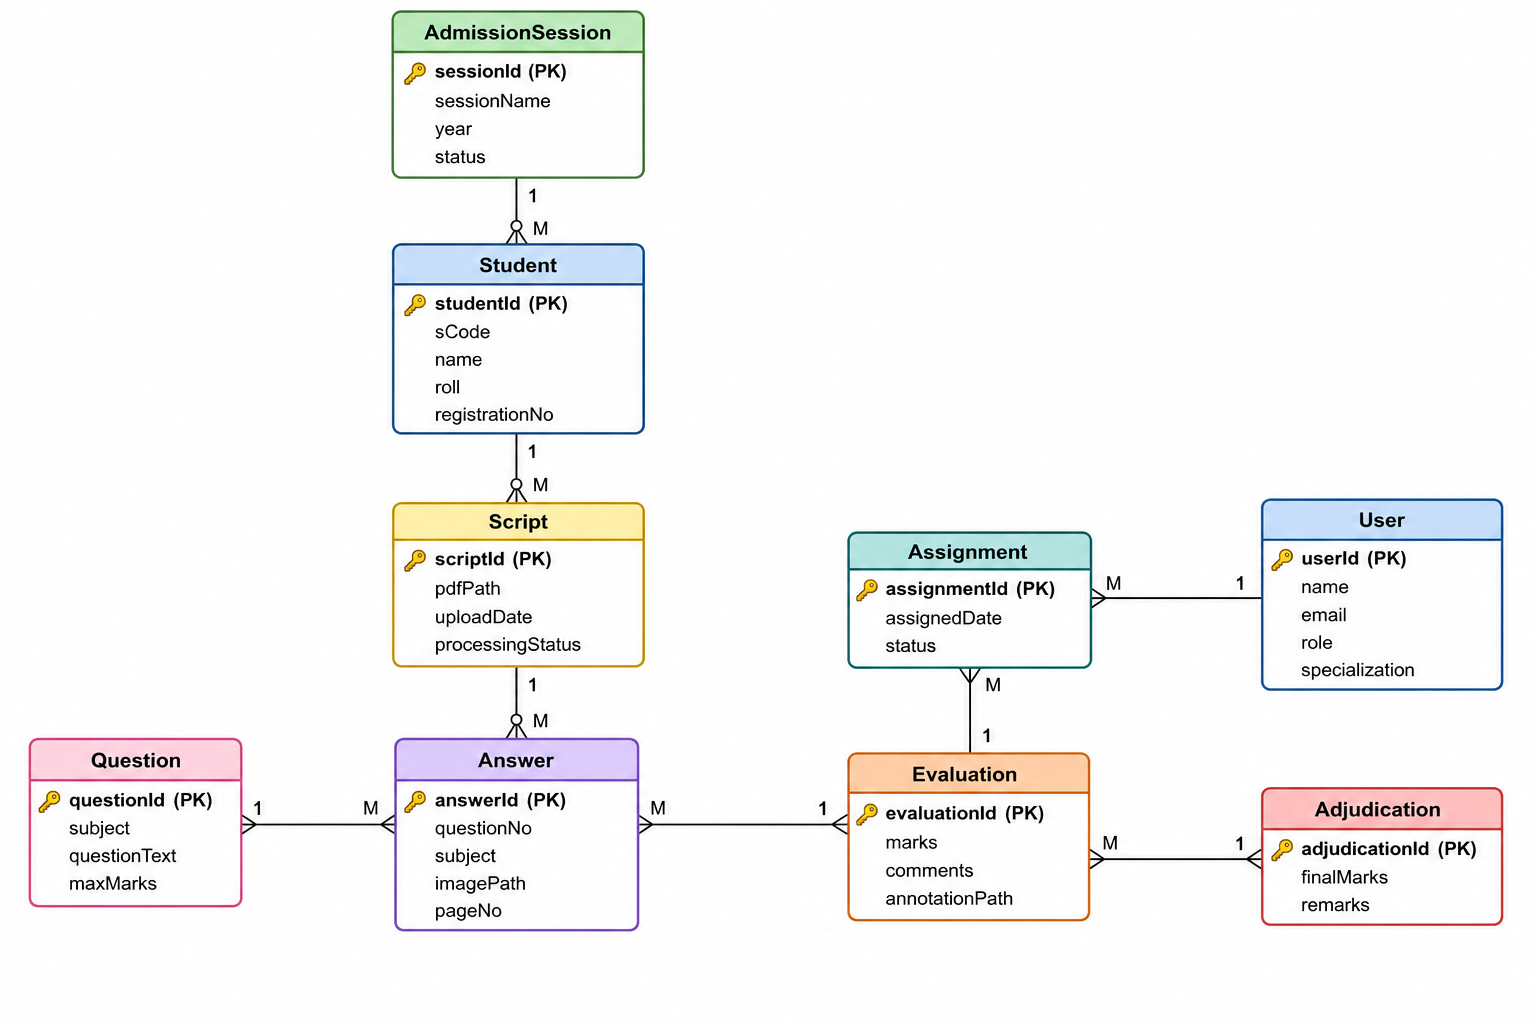
\includegraphics[width=0.90\textwidth]{img/ER_diagram.png}
    \caption{Logical relationships among the primary MongoDB collections.}
    \label{fig:mongodb_relationships}
\end{figure}


\subsubsection{Data Integrity and Consistency}

Mongoose schema validation ensures that all documents satisfy predefined constraints before insertion. Evaluation records remain immutable after submission, while moderation decisions are stored separately to preserve evaluation history. Audit logs follow an append-only strategy, ensuring complete traceability of system activities. Anonymous student identifiers further protect privacy by preventing teachers from accessing personal information during evaluation.

\subsection{PDF Processing Module}

The PDF Processing Module is the core component of the proposed \textbf{Digital Admission Script Evaluation and Moderation System (DASEMS)}. It converts uploaded admission answer scripts into question-wise answer records for digital evaluation. Implemented as an independent Python service, the module performs document validation, page rendering, hybrid question detection, answer extraction, metadata generation, and database integration. By separating document processing from the backend, computationally intensive OCR tasks do not affect application responsiveness.

Unlike conventional OCR-only approaches, the proposed module adopts a hybrid strategy. Searchable PDF text is extracted directly whenever available, while OCR is used only for scanned documents without an embedded text layer. This improves both processing speed and detection accuracy.



% \begin{figure}[ht]
%     \centering
%     \includegraphics[width=0.90\textwidth]{img/pdf_processing_workflow.png}
%     \caption{Implementation workflow of the PDF processing module.}
%     \label{fig:pdf_processing_workflow}
% \end{figure}

\begin{figure}[ht]
\centering

\begin{tikzpicture}[
    node distance=8mm,
    box/.style={
        rectangle,
        rounded corners=6pt,
        minimum width=8cm,
        minimum height=1cm,
        align=center,
        draw=black,
        thick,
        font=\bfseries,
        drop shadow
    },
    line/.style={
        -{Stealth[length=3mm]},
        thick
    }
]

\node[box,fill=blue!15] (A) {PDF Upload};
\node[box,fill=green!15,below=of A] (B) {File Validation};
\node[box,fill=yellow!25,below=of B] (C) {Store Original PDF};
\node[box,fill=orange!25,below=of C] (D) {Render PDF Pages};
\node[box,fill=red!15,below=of D] (E) {Question Detection};
\node[box,fill=purple!15,below=of E] (F) {Answer Region Identification};
\node[box,fill=cyan!20,below=of F] (G) {Answer Image Cropping};
\node[box,fill=pink!20,below=of G] (H) {Metadata Generation};
\node[box,fill=teal!20,below=of H] (I) {Database Storage};

\draw[line] (A) -- (B);
\draw[line] (B) -- (C);
\draw[line] (C) -- (D);
\draw[line] (D) -- (E);
\draw[line] (E) -- (F);
\draw[line] (F) -- (G);
\draw[line] (G) -- (H);
\draw[line] (H) -- (I);

\end{tikzpicture}

\caption{PDF Processing Workflow}
\label{fig:pdf_workflow}

\end{figure}



\subsubsection{PDF Upload and Validation}

The uploaded PDF is validated for file integrity, format, and readability before processing. Each document is linked to the corresponding admission session and anonymous student identifier (\textbf{s\_code}), while the original PDF is stored without modification to preserve authenticity throughout the evaluation process.

\subsubsection{PDF Rendering}

Each PDF page is converted into a high-resolution image using PyMuPDF. These rendered images provide a standardized input for OCR and subsequent image-processing operations while preserving the original document layout.

\subsubsection{Hybrid Question Detection}

The processor first attempts to extract embedded text directly from the PDF. If searchable text is unavailable, OCR is applied to detect printed question numbers and their coordinates. This hybrid approach ensures reliable processing for both digitally generated and scanned answer scripts while minimizing unnecessary OCR operations.



\begin{figure}[H]
    \centering
    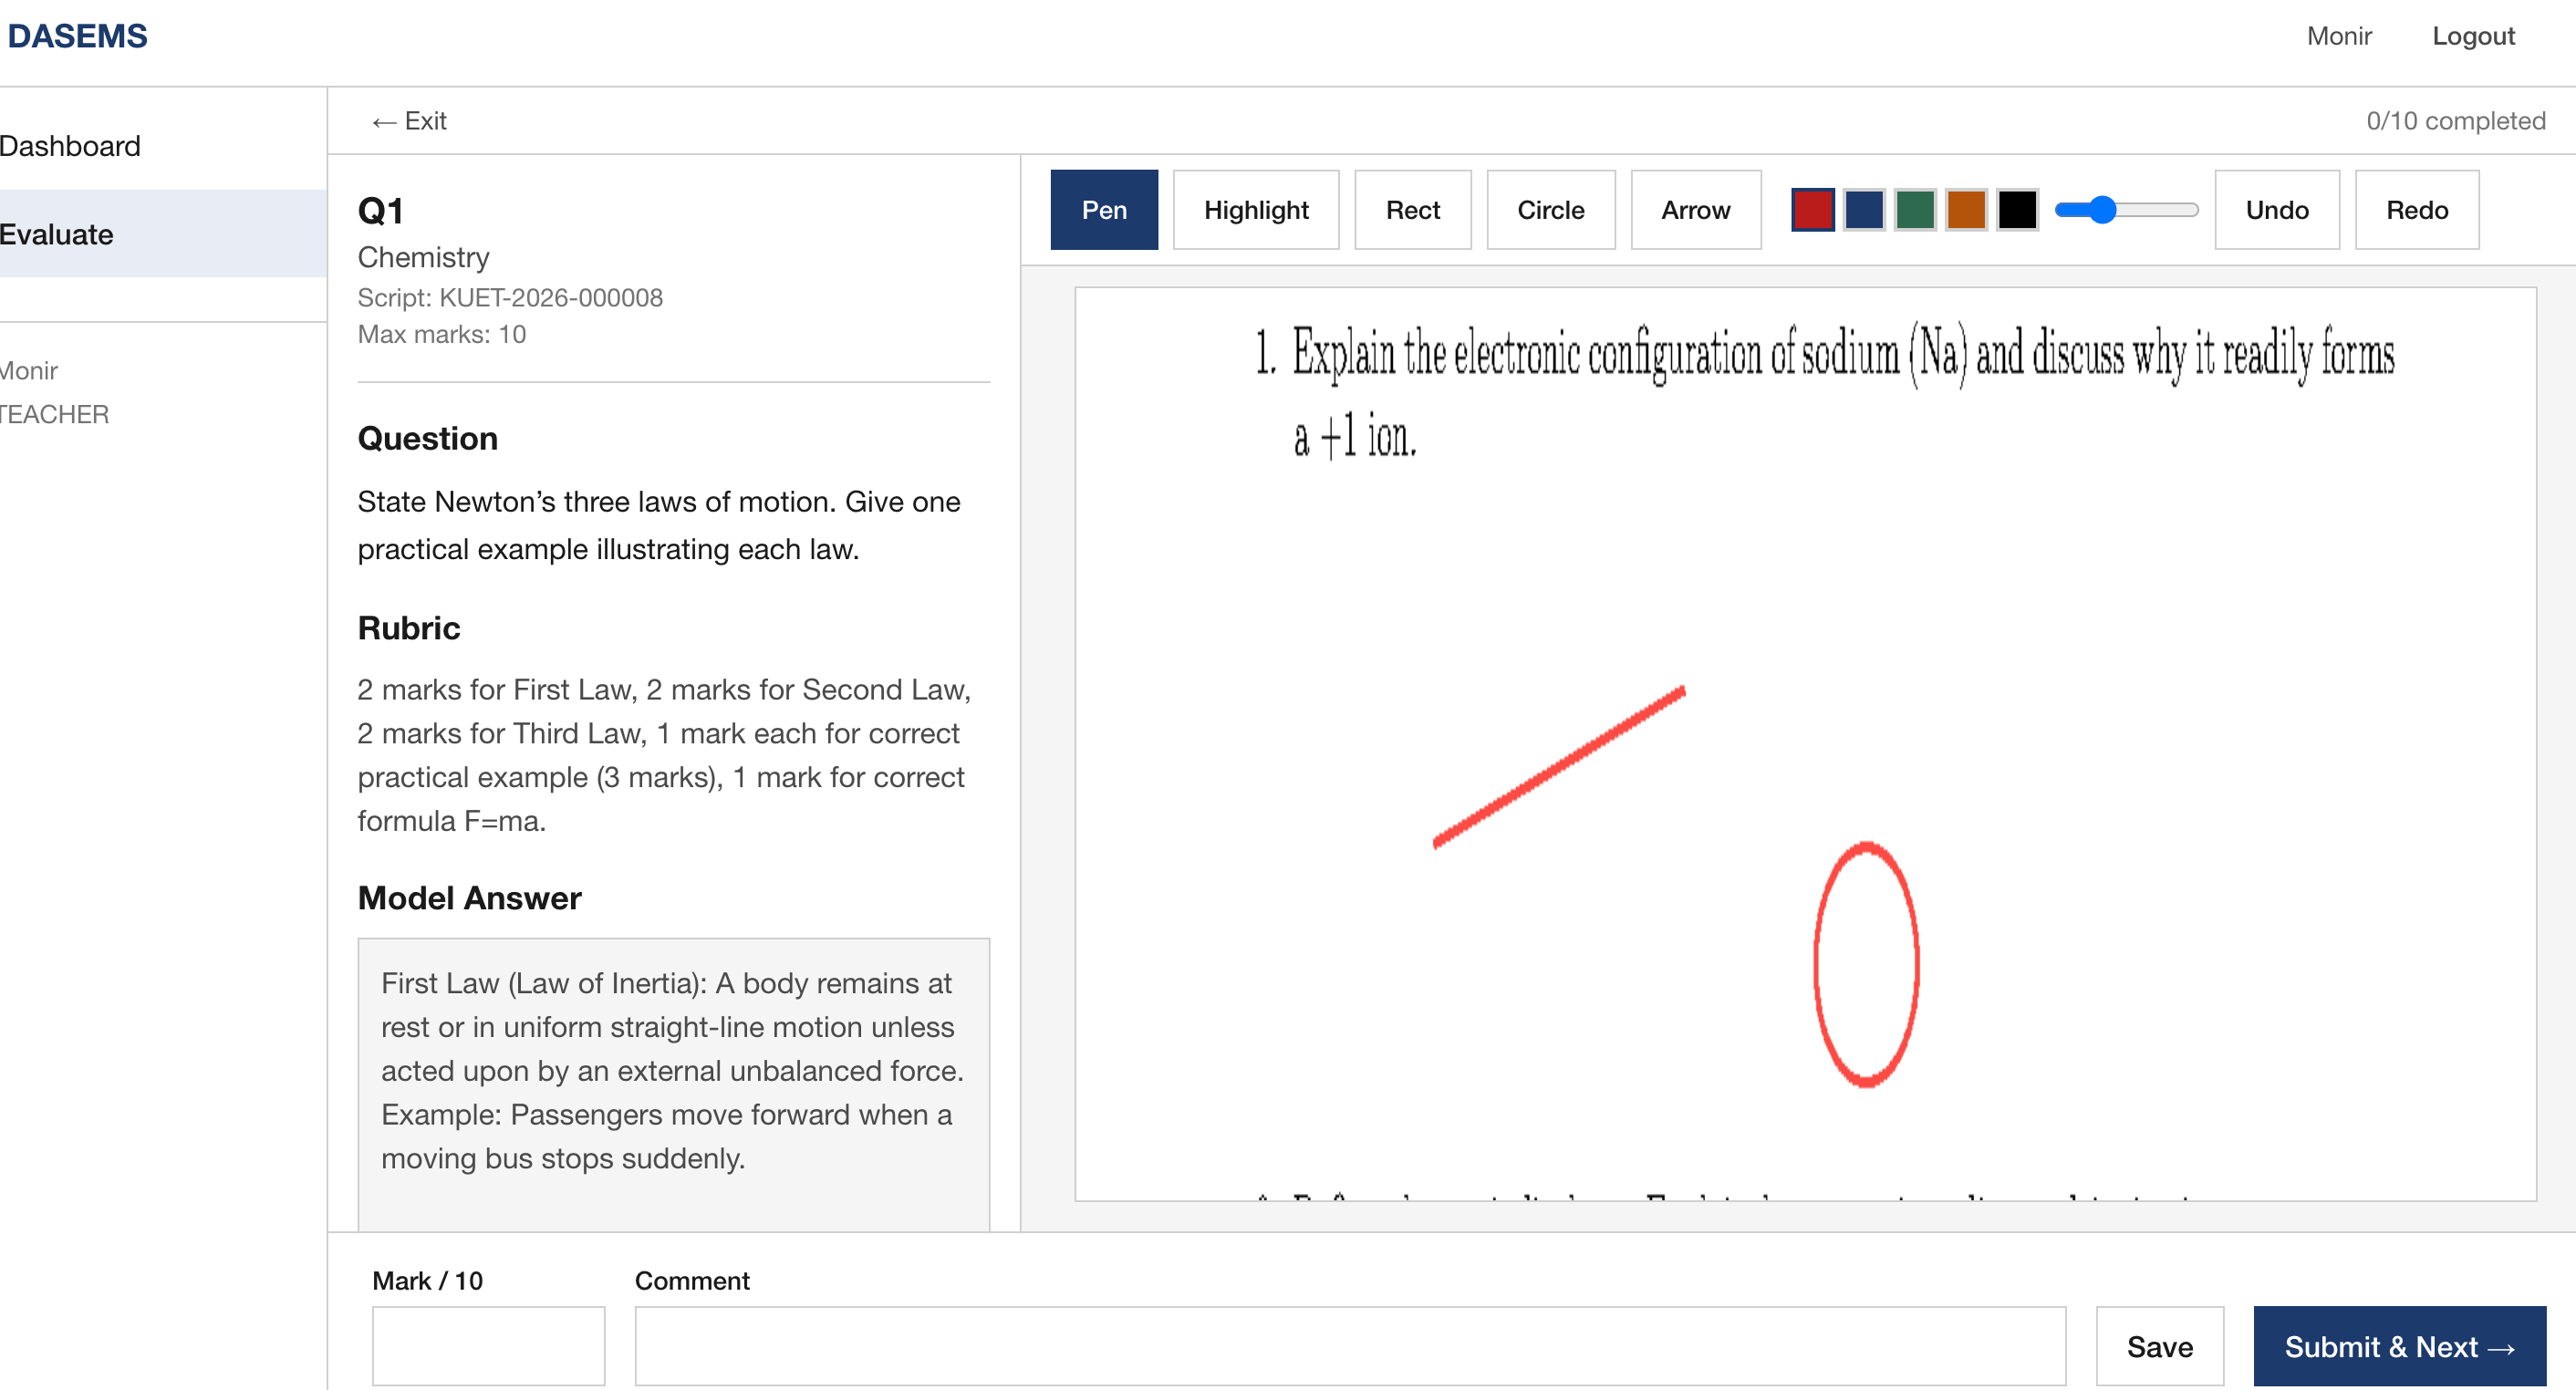
\includegraphics[width=0.90\textwidth]{img/question_detection.png}
    \caption{Hybrid question detection using PDF text extraction and OCR.}
    \label{fig:question_detection}
\end{figure}

\subsubsection{Answer Region Identification}

Using the detected question positions, the processor dynamically determines answer boundaries. Each answer begins below its corresponding question and extends to the next detected question or the end of the page. Multi-page answers are handled automatically, allowing answers of varying lengths to be extracted correctly.



\begin{figure}[H]
    \centering
    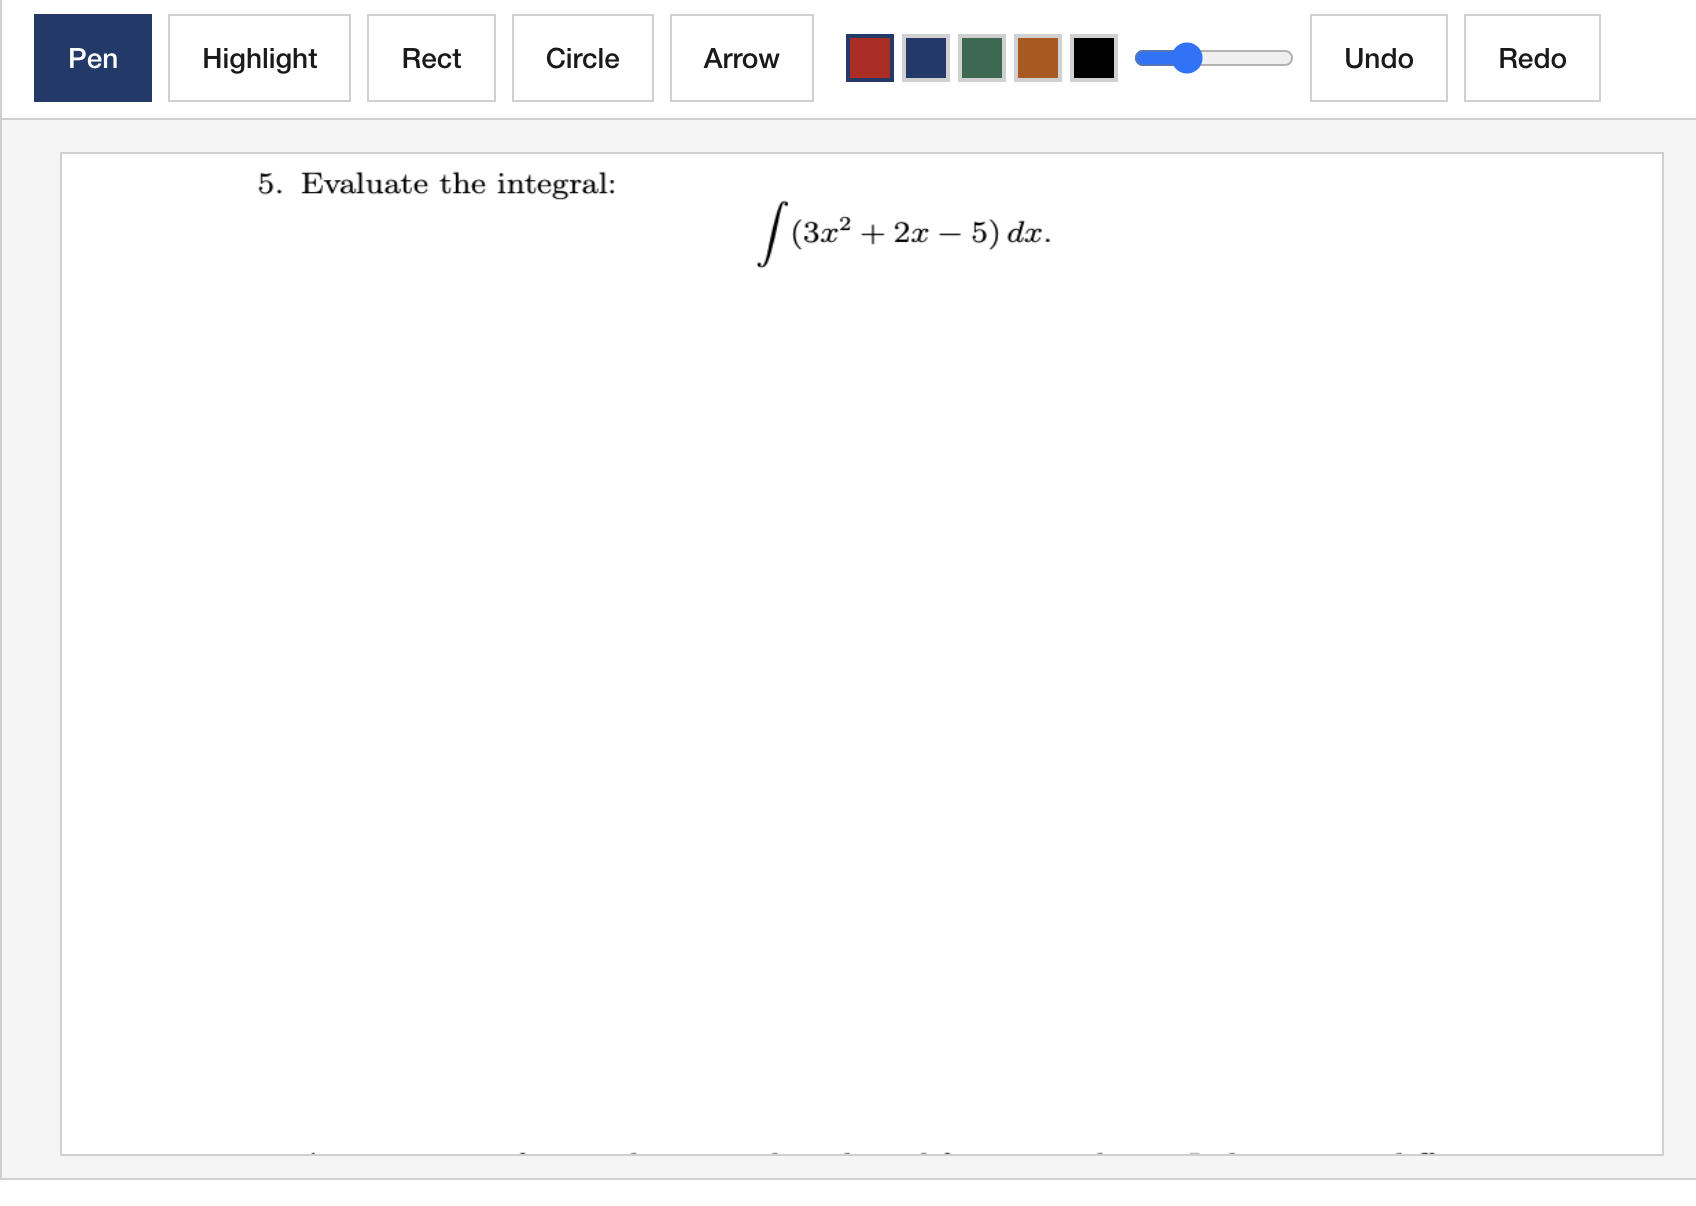
\includegraphics[width=0.85\textwidth]{img/question_detection1.png}
    \caption{Dynamic identification of answer boundaries based on detected question positions.}
    \label{fig:answer_segmentation}
\end{figure}

\subsubsection{Answer Extraction and Metadata Generation}

The identified answer regions are cropped using the Pillow library and stored as independent images. For each extracted answer, the processor generates metadata including the anonymous student identifier, subject, question number, page number, bounding coordinates, image location, and processing status. The metadata are transmitted to the backend as JSON objects for database storage and automatic teacher assignment.

\subsubsection{Database Integration}

The backend creates an independent database record for every extracted answer. Each record stores the extracted image reference, metadata, and processing status. These records serve as the primary evaluation units and are subsequently used for teacher assignment, evaluation, moderation, and result generation.

\subsubsection*{Algorithm 4.1: PDF Processing Pipeline}

\begin{verbatim}
Input:
    Uploaded PDF Document

Output:
    Question-wise Answer Records

Begin

Receive uploaded PDF
Validate document
Store original PDF
Render pages

For each page do

    Extract PDF text

    If unavailable
        Perform OCR
    End If

    Detect questions
    Determine answer boundaries
    Crop answers
    Generate metadata

End For

Store answer records
Return processing status

End
\end{verbatim}


\subsection{Teacher Assignment and Evaluation Implementation}

The proposed \textbf{Digital Admission Script Evaluation and Moderation System (DASEMS)} implements an automated teacher assignment mechanism to ensure fair, anonymous, and balanced evaluation of descriptive answers. After the PDF processing module extracts question-wise answers, the backend retrieves the associated metadata, including subject, question number, anonymous student identifier (\textbf{s\_code}), and answer image location. Based on the subject, the system automatically assigns answers to qualified teachers without manual intervention.

The assignment engine selects teachers according to their subject specialization and current evaluation workload to ensure balanced distribution. 

To maintain fairness, teachers evaluate answers using only the anonymous student identifier. The evaluation interface provides the extracted answer image, question statement, model answer, marking rubric, annotation tools, and mark submission form. Once submitted, evaluation records become read-only unless modified through the moderation process.

% for figure: 
\begin{figure}[H]
\centering

\begin{tikzpicture}[
    node distance=0.9cm,
    >=Stealth,
    process/.style={
        rectangle,
        rounded corners=8pt,
        draw=black!70,
        very thick,
        minimum width=8cm,
        minimum height=1cm,
        align=center,
        font=\bfseries,
        drop shadow
    },
    arrow/.style={
        ->,
        very thick,
        >=Stealth
    }
]

\node[process,fill=box1] (A) {Extracted Answer};

\node[process,fill=box2,below=of A] (B)
{Identify Subject};

\node[process,fill=box3,below=of B] (C)
{Retrieve Eligible Teachers};

\node[process,fill=box4,below=of C] (D)
{Check Current Workload};

\node[process,fill=box5,below=of D] (E)
{Assign to Three Teachers};

\node[process,fill=box6,below=of E] (F)
{Create Assignment Records};

\node[process,fill=box7,below=of F] (G)
{Teacher Evaluation Queue};

\draw[arrow] (A) -- (B);
\draw[arrow] (B) -- (C);
\draw[arrow] (C) -- (D);
\draw[arrow] (D) -- (E);
\draw[arrow] (E) -- (F);
\draw[arrow] (F) -- (G);

\end{tikzpicture}

\caption{Teacher Assignment Workflow}
\label{fig:teacher_assignment_workflow}

\end{figure}
\FloatBarrier




\subsubsection{Moderation Implementation}

To improve evaluation consistency, the system automatically compares the marks submitted by the three evaluators. If the difference between the highest and lowest marks is within the predefined moderation threshold, the final score is calculated as the average of the submitted marks.

When the variation exceeds the threshold, the answer is forwarded to the Head Examiner for moderation. The moderation dashboard displays the extracted answer image, model answer, marking rubric, teacher marks, comments, and annotations. After reviewing these materials, the Head Examiner assigns the final mark, which is permanently stored together with moderation remarks and timestamps.

The automated assignment and moderation mechanisms reduce administrative effort while improving fairness, transparency, and consistency throughout the admission evaluation process.



\subsection{Result Generation}

After teacher evaluation and moderation are completed, the proposed \textbf{Digital Admission Script Evaluation and Moderation System (DASEMS)} automatically generates the final admission examination results. The result generation module consolidates finalized evaluations, calculates student scores, and prepares administrative reports, thereby reducing manual effort and calculation errors.

Before generating results, the system verifies that all assigned evaluations and moderation tasks have been completed. If any answer remains pending, the corresponding student's result is withheld until the evaluation process is finalized. Once all evaluations are complete, the backend retrieves the approved marks for each question and automatically calculates the total score according to the examination rules.

% Figure~\ref{fig:result_generation} illustrates the workflow of the result generation module.

% \begin{figure}[ht]
%     \centering
%     \includegraphics[width=0.85\textwidth]{img/result_generation_workflow.png}
%     \caption{Workflow of the result generation module.}
%     \label{fig:result_generation}
% \end{figure}




The generated results are stored in the MongoDB database and displayed through the administrative dashboard. Administrators can access merit lists, subject-wise performance summaries, and complete evaluation histories for verification.

The reporting module also provides statistics such as:

\begin{itemize}
    \item Total evaluated answer scripts.
    \item Pending evaluations.
    \item Moderated answers.
    \item Subject-wise performance.
    \item Teacher workload.
    \item Final examination results.
\end{itemize}

By combining automatic score calculation with centralized reporting, the implemented module improves the efficiency, accuracy, and transparency of the admission evaluation process.


\subsection{System Testing and Validation}

After implementing all software modules, comprehensive testing was conducted to verify the correctness, reliability, and integration of the proposed \textbf{Digital Admission Script Evaluation and Moderation System (DASEMS)}. The testing process ensured that each module satisfied the functional requirements identified during system analysis.

Initially, unit testing was performed on individual modules, including authentication, admission management, PDF processing, answer extraction, teacher assignment, evaluation, moderation, and result generation. Integration testing was then conducted to verify communication among the React frontend, Node.js backend, Python document processing service, and MongoDB database.

Table~\ref{tab:functional_testing} summarizes the functional testing results.

\begin{table}[ht]
\centering
\caption{Functional Testing Results}
\label{tab:functional_testing}

\begin{tabular}{|p{6cm}|p{6cm}|p{2cm}|}
\hline
\textbf{System Function} & \textbf{Expected Outcome} & \textbf{Result} \\
\hline
User Login & Authorized user access & Pass \\
\hline
JWT Authentication & Secure API access & Pass \\
\hline
Admission Session Creation & Session stored successfully & Pass \\
\hline
Question Upload & Questions imported correctly & Pass \\
\hline
Student Registration & Student information stored & Pass \\
\hline
PDF Upload & Document accepted and stored & Pass \\
\hline
PDF Processing & Questions detected successfully & Pass \\
\hline
Answer Extraction & Answer images generated & Pass \\
\hline
Teacher Assignment & Subject-based assignment completed & Pass \\
\hline
Evaluation Submission & Marks stored successfully & Pass \\
\hline
Moderation Workflow & Head Examiner review activated & Pass \\
\hline
Result Generation & Final marks calculated correctly & Pass \\
\hline
\end{tabular}

\end{table}

The testing results confirm that all modules function correctly and interact successfully within the integrated system. Uploaded answer scripts progressed through the complete workflow, including PDF processing, teacher assignment, evaluation, moderation, and result generation.

Usability testing was also performed using different user roles. Super Administrators successfully managed examination data and generated reports, Teachers evaluated assigned answers through the browser-based interface, and Head Examiners completed moderation using the dedicated dashboard.

Performance testing showed that separating OCR into an independent Python service prevented document processing from affecting frontend responsiveness, allowing multiple users to access the system efficiently.

Overall, the testing process demonstrates that the implemented DASEMS satisfies the functional requirements and provides a reliable platform for descriptive university admission examinations.


\subsection{Chapter Summary}

This chapter presented the implementation of the proposed \textbf{Digital Admission Script Evaluation and Moderation System (DASEMS)}. The system was developed as a modular web-based platform using React, Node.js, MongoDB, and a Python-based document processing service. This architecture provides a scalable and maintainable solution for managing descriptive admission script evaluation.

The implementation included secure authentication, role-based access control, admission management, PDF processing, automated teacher assignment, digital evaluation, moderation, audit logging, and result generation. A hybrid PDF processing pipeline combining embedded text extraction and OCR was implemented to identify question boundaries and generate question-wise answer images for evaluation.

The chapter also demonstrated how automated teacher assignment, anonymous evaluation, and moderation improve fairness and reduce administrative effort. Functional and integration testing confirmed that all modules operate correctly and communicate successfully within the integrated architecture.

Overall, the implemented system provides a reliable digital framework for descriptive admission script evaluation while supporting future enhancements such as AI-assisted handwriting recognition and cloud-based deployment.

The next chapter presents the experimental evaluation of the proposed system, including performance analysis, functional validation, and discussion of the implementation results.

